\chapter*{Ringraziamenti}
\addcontentsline{toc}{chapter}{Ringraziamenti}
\vspace{-8mm}
Questa tesi è stata resa possibile dal contributo nella mia vita di tante persone, che giorno per giorno mi hanno sempre dato il loro sostegno, a voi dedico questa mia Tesi.\\
Un ringraziamento speciale alla mia famiglia, in particolare a mia \textbf{Madre} e mio \textbf{Padre}: è grazie al vostro sostegno e incoraggiamento se oggi sono riuscito a raggiungere questo traguardo.\\
La forza di arrivare qui, oggi, però non è dovuta solo a loro, devo per forza ringraziare dell'affetto e il sostegno speciale da parte dei miei cari amici, che ogni giorno hanno condiviso con me gioie, sacrifici e successi, senza voltarmi mai le spalle, mi hanno dato la forza di arrivare a questo prezioso traguardo. \textbf{Filippo}, \textbf{Gabriele}, \textbf{Marta}, grazie di TUTTO.\\
Un pensiero in particolare vola verso la mia dolce \textbf{\textit{Nicoleta}}, è sicuramente grazie all'affetto e le attenzioni che mi hai donato che sono riuscito a tenere dritto il timone ed arrivare qui oggi.
Per terminare voglio ringraziare tutti i professori che negli ultimi 18 anni hanno guidato il mio cammino, loro che hanno sempre creduto in me e nelle mie capacità meritano tutta la mia gratitudine.\\
Un ringraziamento speciale va però alla mia professoressa e mentore \textbf{Beniamina Rauch} che fu la prima a vedere il mio potenziale e coltivarlo, so che ancora vegli su di me, non troverò mai le parole per ringraziarti abbastanza.\\
Oltre a lei ringrazio il mio relatore \textbf{Daniele Carnevale} che in questi anni universitari, da quando mi ha conosciuto ad oggi, ha sempre creduto in me e mi ha permesso di fare esperienze che mai avevo immaginato.\\ \\
Un sentito grazie a tutti voi e buona lettura.


\chapter*{Introduzione}
\addcontentsline{toc}{chapter}{Introduzione}
La tesi si colloca nell'ambito delle tecniche di controllo per impianti Tokamak, come FTU (Frascati Tokamak Upgrade), Proto-Sphera ed ITER (International Thermonuclear Experimental Reactor).\\
Essa è stata realizzata in collaborazione con il centro ricerche \textbf{ENEA} (Ente Nazionale per l’Energia e l’Ambiente) di Frascati e coordinato dal gruppo \textbf{CODAS} (COntrol and Data Acquisition System).\\
L'obiettivo finale del CODAS è di gestire il sistema di controllo ed acquisizione di un intero impianto Tokamak.\\
In questa tesi viene discussa la creazione e lo sviluppo del prototipo dell'architettura e le leggi di controllo per l'asservimento della corrente nelle bobine magnetiche, generando così il confinamento magnetico del Plasma necessario alla reazione di fusione nucleare, che avviene all'interno del Tokamak.
\newpage

\section*{Struttura di un Tokamak}
\addcontentsline{toc}{section}{Struttura di un Tokamak}
Un \textbf{Tokamak}\footnote{Tokamak è l'acronimo russo per "camera toroidale magnetica"} è una macchina di forma toroidale (a ciambella) in cui un gas (solitamente idrogeno) viene portato nello stato di Plasma e mantenuto coeso e lontano dalle pareti interne grazie ad un campo magnetico creato da elettromagneti esterni alla camera.\\
Scopo di un Tokamak è generare in maniera controllata reazioni di \textbf{fusione nucleare}.\\
\begin{figure}[H]
	\centering
	\caption[Sezione di un Tokamak]{Sezione di un Tokamak}
	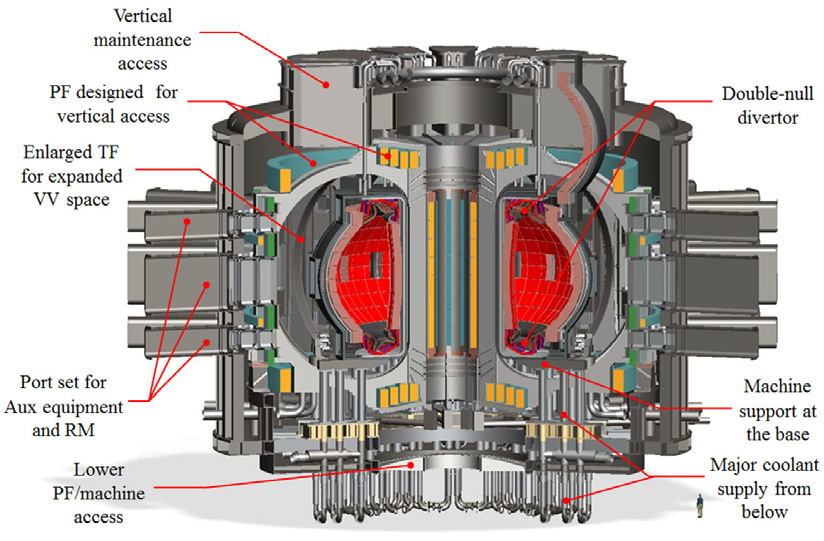
\includegraphics[width=0.65\textwidth]{Introduzione/K-DEMO_device_core_design_features.jpg}
\end{figure}

\noindent
La forma del Tokamak a \textit{toro} è studiata per permettere alle particelle del Plasma di muoversi all'interno del campo magnetico, creato all'esterno delle pareti (\textit{Esterno del Vessel}) in un moto circolare.\\
Questo movimento avviene poiché le particelle del Plasma sono per definizione cariche, e in quanto tali, se immerse in un campo magnetico esse tendono a muoversi seguendo una traiettoria elicoidale (detta anche \textit{moto di ciclotrone}) attorno alle linee del campo magnetico, che in questo caso sono chiuse e contenute all'interno della sezione del Tokamak (\textit{Interno del Vessel}).\\
L'uso di una confinazione magnetica di questo Plasma è dovuta all'impossibilità, per qualunque materiale, di resistere alle enormi temperature raggiunte dal Plasma durante la fusione in caso di un contatto diretto.\\

\noindent
La forma scelta per i Tokamak a Toro ha motivazioni fisiche, che discendono principalmente dall'equazione di Larmor. L'equazione descrive la distanza massima oltre il quale una particella carica non può allontanarsi da una linea di campo magnetico, definendo un limite superiore per lo spazio di contenimento delle particelle; questa distanza è detto appunto \textit{raggio di Larmor}:\\
\begin{vwcol}[widths={0.3,0.7}, sep=8mm, rule=1px]
	\begin{empheq}[box=\mathCalc]{equation*} \label{eq:Larmor}
		{\displaystyle \,\rho ={\frac {mv_{\perp }}{Ze\,B}}}
	\end{empheq}
	\newpage % con wcol, le colonne sono "pagine"
	\begin{spacing}{1.25}
		{\footnotesize
			$ {\displaystyle v_{\perp }} $ è la velocità della particella perpendicolare al campo magnetico.\\
			$ {\displaystyle m} $ è la sua massa.\\
			$ {\displaystyle B} $ è l'intensità del campo magnetico.\\
			$ {\displaystyle Ze} $ è la carica del portatore.
		}
	\end{spacing}
\end{vwcol}
\noindent
L'equazione vale anche in presenza di un campo magnetico curvo, se questa curva è chiusa si ottiene che la particella è confinata in uno spazio di volume finito ma rimane comunque libera ruotare all'infinito, accumulando così energia.\\
\'E stata scelta la geometria del \textbf{Toro} per rendere questa linea di campo una circonferenza esatta, la quale semplifica enormemente delle complesse equazioni fluido-dinamiche applicate al Plasma.\vspace{-5mm}
\begin{figure}[H]
	\centering
	\caption[Geometria di un Toro]{Geometria di un Toro}
	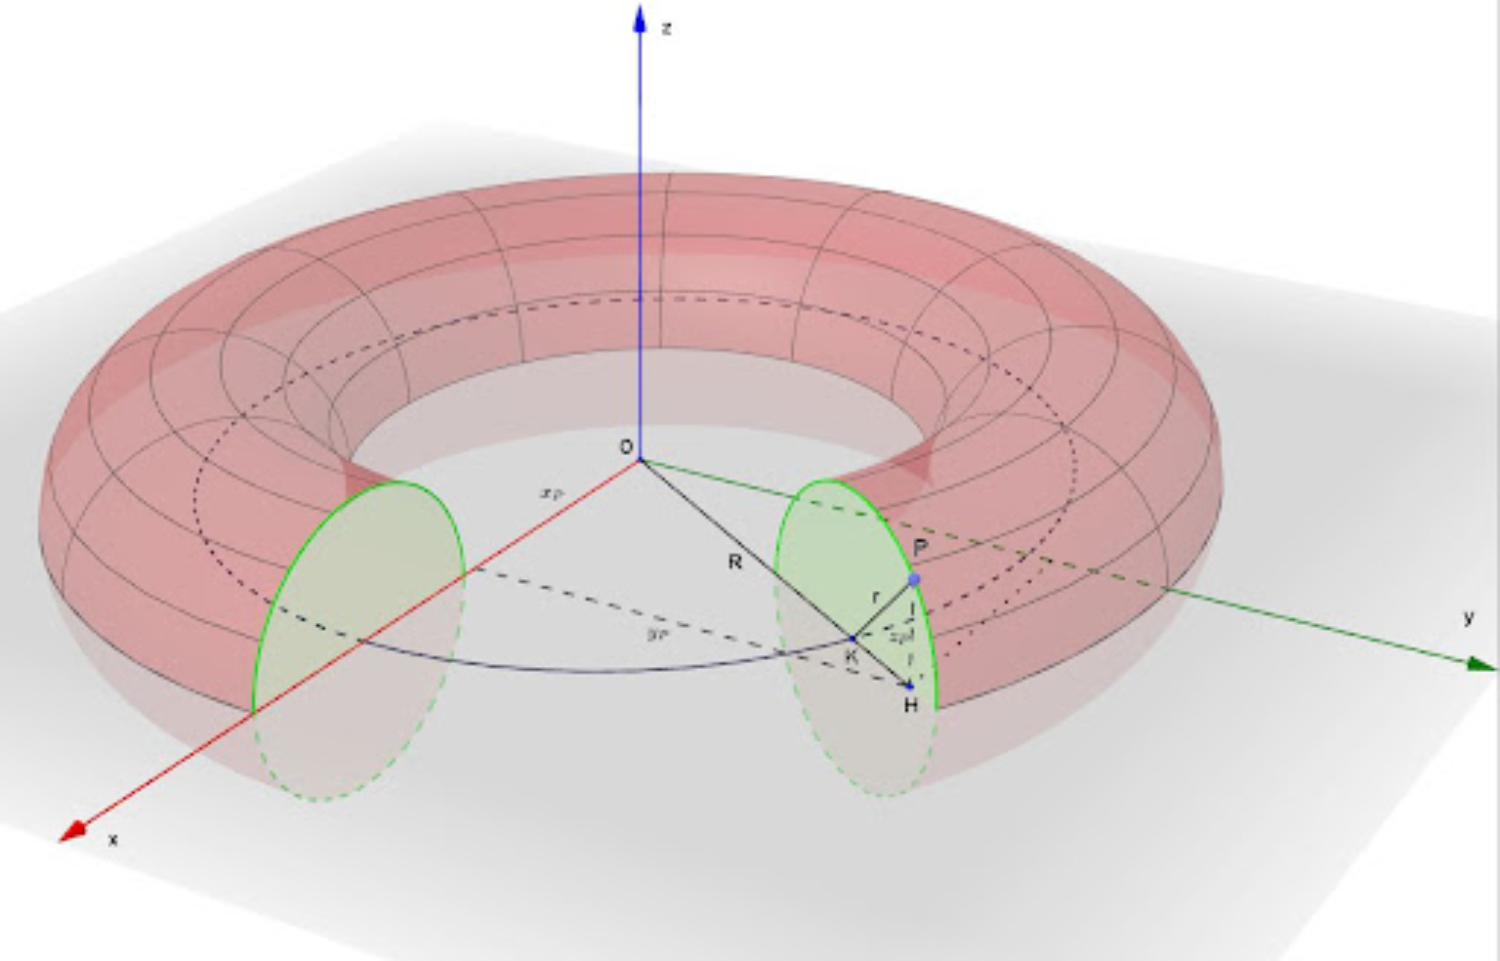
\includegraphics[width=0.65\textwidth]{Introduzione/toro-big.png}
\end{figure}\vspace{-8mm}
\noindent
In sintesi un Tokamak è un impianto progettato per creare questo confinamento magnetico in maniera efficace e sicura, e ha la forma più consona per realizzare questo processo.\\
Oltre al mero contenimento però, il secondo obiettivo è quello di compattare il Plasma su se stesso (aumentando la forza del campo magnetico $ B $), così da avvicinare di più gli atomi tra loro (l'aumento di $ B $ causa una riduzione di $ \rho $).\\
Questo aumento di pressione, unito alle alte energie immesse nel Tokamak (la cui temperatura è \textbf{di decine di volte} superiore a quella della superficie del sole) aumentano le probabilità di scontro tra gli atomi, e quindi inizio di un processo di fusione tra essi. 

\newpage

\section*{Cos'è la Fusione Termonucleare?}
\addcontentsline{toc}{section}{Cos'è la Fusione Termonucleare?}
In fisica, per \textbf{Fusione Termonucleare}, si intende il processo mediante il quale i nuclei di due o più atomi vengono compressi tanto da far prevalere l’interazione forte sulla repulsione coulombiana, causando l'unione tra gli atomi e andando a formare così un nucleo la cui massa totale risulta minore della massa dei reagenti originali. La perdita di massa ha come conseguenza la liberazione di un’elevata quantità di energia, la quale conferisce al processo caratteristiche fortemente esotermiche.\\
La massa mancante viene trasformata in energia in accordo con l’equazione di Einstein:
\begin{center}
	$E = (m_r - m)c^2$
\end{center}
Dove $ m_r $ è la massa dei reagenti e $ m $ è la massa risultante.\\
Il processo di \textbf{fusione nucleare} avviene naturalmente all'interno delle stelle e trasforma l'\textit{idrogeno} (di cui sono composte) in \textit{elio}.\\
L'energia nucleare prodotta a seguito di questa reazione è elevatissima e per tale motivo risulta di forte interesse per la civiltà umana sviluppare tecniche sofisticate che ne permettano la raccolta in maniera controllata.\\
Tra i vantaggi di questa tecnologia troviamo sia motivi economici che ambientali e i principali possono essere sintetizzati in:
\begin{description}
	\item [Combustibile semi-inesauribile:]\phantom{.}\\
	      Il combustibile (idrogeno e/o deuterio) è praticamente inesauribile ed è a disposizione di tutte le nazioni che abbiano uno sbocco sul mare. Il deuterio può essere estratto dall'acqua, anche se con costi energetici non indifferenti;\\
	      per fare un esempio, un ditale pieno di deuterio equivale a 20 tonnellate di carbone in termini di energia.\\
	      Un lago di medie dimensioni contiene deuterio sufficiente a rifornire una nazione di energia per secoli utilizzando la fusione nucleare (ovviamente supponendo di sfruttarlo tutto).
	\item [Rischi di Contaminazione grave sono \underline{nulli}:]\phantom{.}\\
	      Nessuna possibilità di incidenti come quelli di Černobyl' o di Three Mile Island in quanto il reattore non contiene sostanze radioattive come l'uranio o le scorie di fissione.\\
	      In oltre, possibili incidenti, come fughe di trizio o perdite di liquido refrigerante, avrebbero un impatto ambientale e radiativo molto più contenuto e temporaneo.
	\item [Assenza di inquinanti ambientali:]\phantom{.}\\
	      Il processo di fusione, durante il quale gli atomi di idrogeno vengono fusi per creare elio, non rilascia nessun elemento inquinante da combustione (ad esempio anidride carbonica) e per tanto nessun residuo può essere immesso nell'atmosfera impedendo il riscaldamento del pianeta tramite l'effetto serra.
	\item [Nessuno prodotto derivato è adatto a fini Bellici:]\phantom{.}\\
	      La mancanza di materiale radioattivo residuo, impedisce l'utilizzo dei reattori per la produzione di materiale per scopi bellici o terroristici, come proiettili radioattivi o materiale fissile per bombe nucleari.
	\item [Livelli lievi di radioattività residua:]\phantom{.}\\
	      Il processo di fusione può rendere radioattivi solo i materiali che compongono il Tokamak e i gas usati per il Plasma, ma entrambi gli elementi possiedono un tempo di decadimento alquanto breve, il ché implica che i rifiuti radioattivi hanno una scarsa durata nel tempo, in oltre le radiazioni prodotte non sono a energie elevatissime, semplificandone il contenimento attraverso contenitori schermati più economici e sicuri.
\end{description}
\noindent
Questi e molti altri motivi rendono lo sviluppo di metodi per catturare l'energia da \textbf{Fusione Nucleare} con attraverso processi controllati di grande interesse per tutta la civiltà umana, essa potrebbe infatti essere la chiave per preservare l'ambiente del nostro pianeta e fornire al temo stesso l'energia di cui l'umanità necessita.\\
In questa tesi faremo riferimento ad una classe di impianti sperimentali per la \textbf{Fusione Nucleare Controllata}, detti "\textbf{Impianti Tokamak}". \'E doveroso specificare che essi sono solo uno dei tanti design su cui attualmente si fa ricerca e sviluppo nel mondo, ma tra le varie proposte essi sembrano essere i più promettenti per aprire le porte a questa rivoluzione, poiché il principio di base è la replica delle condizioni che generano la fusione all'interno in una stella.\\
Tolte le difficoltà tecniche per le quali infatti è ancora una tecnologia in sviluppo, abbiamo la sicurezza sperimentale della fattibilità del processo, la nostra stessa civiltà non esisterebbe se il Sole non producesse questa forma di energia al suo interno.
\newpage


\section*{Obiettivi della Tesi}
\addcontentsline{toc}{section}{Obiettivi della Tesi}
Il progetto complessivo portato avanti dall'ENEA prevede la realizzazione di prototipi a più livelli di un sistema Tokamak.\vspace{-4mm}
\begin{figure}[H]
	\centering
	\caption[Architettura Complessiva Progetto ENEA]{Architettura Complessiva Progetto ENEA}
	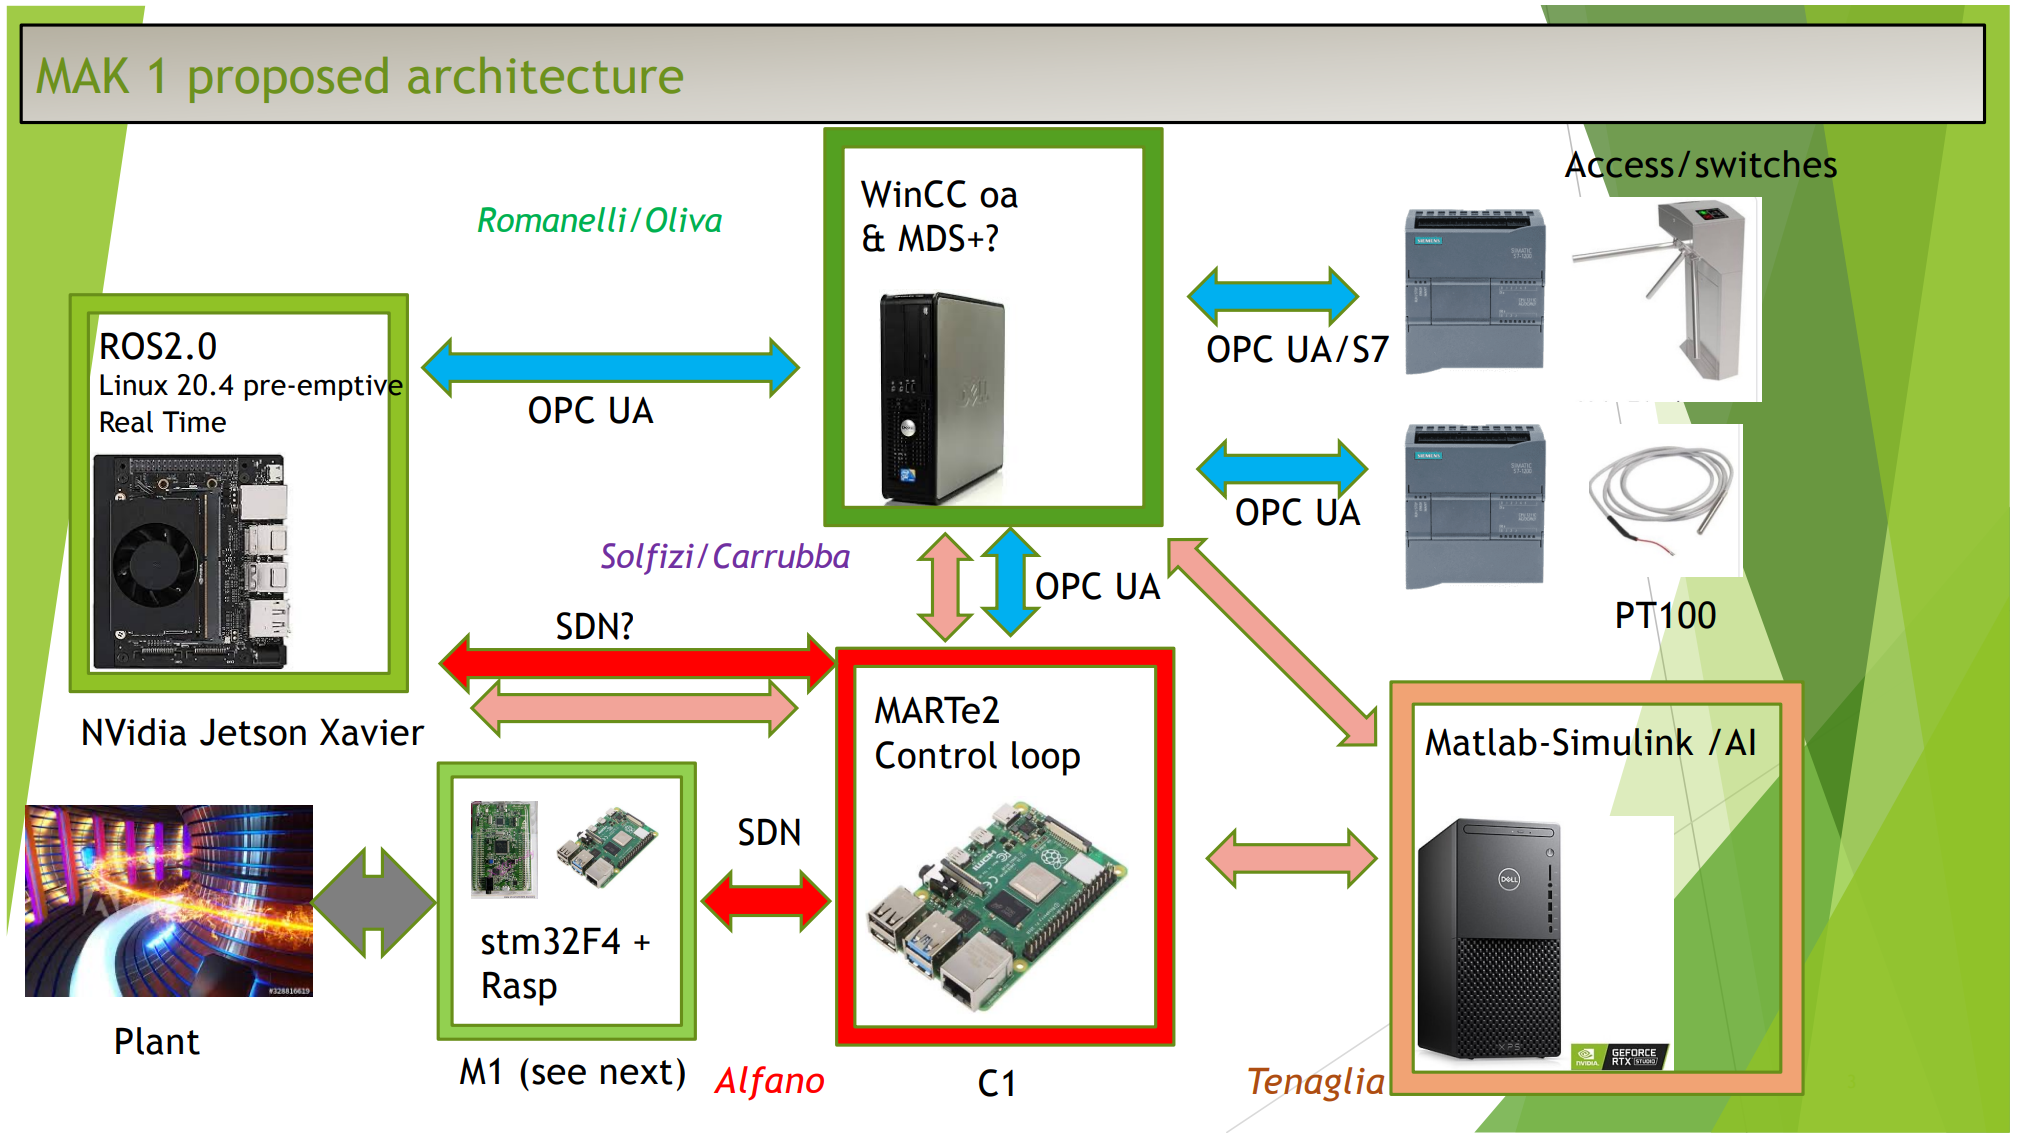
\includegraphics[width=\textwidth]{Introduzione/ArchitetturaComplessiva.png}
\end{figure}\vspace{-8mm}
\noindent
La mia parte di progetto ({\color{red}Alfano}) consiste nello sviluppare e realizzare una una scheda embedded.\\
Essa dovrà pilotare la corrente nelle bobine dell'impianto Tokamak ed essere in grado di ricevere e inseguire i riferimenti per la corrente di Plasma attraverso la rete di interconnessione tra i dispositivi, basata sul Framework di \MARTe. (argomento trattato con dettaglio nella tesi)\\
Il controllo realizzato punta a inseguire il riferimento richiesto con un errore nullo.\\
In fine il dispositivo deve essere in grado di comunicare in real-time l'attuale stato del sistema al resto della rete, per permettere una diagnostica in tempo reale dell'andamento dell'impianto.\\